\chapter{Resultados}
\label{chap_resultados}

Neste capitulo sao apresentados resultados qualitativos (figuras de evolucao) e quantitativos (metricas calculadas a partir dos dados de saida em CSV).

\section{Regras representativas por classe}

As Figuras~\ref{fig:homogeneo-r0} a~\ref{fig:complexo-r110} mostram duas regras por classe de Wolfram, todas com \(tamanho=101\) e \(passos=100\).

\begin{figure}[H]
    \centering
    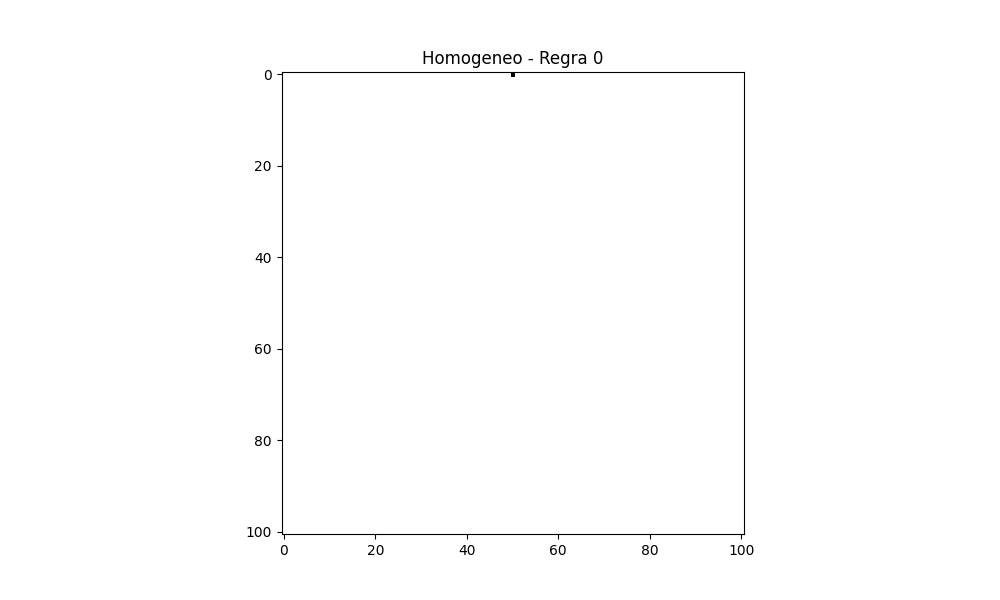
\includegraphics[width=0.75\textwidth]{figuras/graficos/Homogeneo_regra_0_tamanho_101_passos_100.png}
    \caption{Classe homogenea: Regra 0.}
    \label{fig:homogeneo-r0}
\end{figure}

\begin{figure}[H]
    \centering
    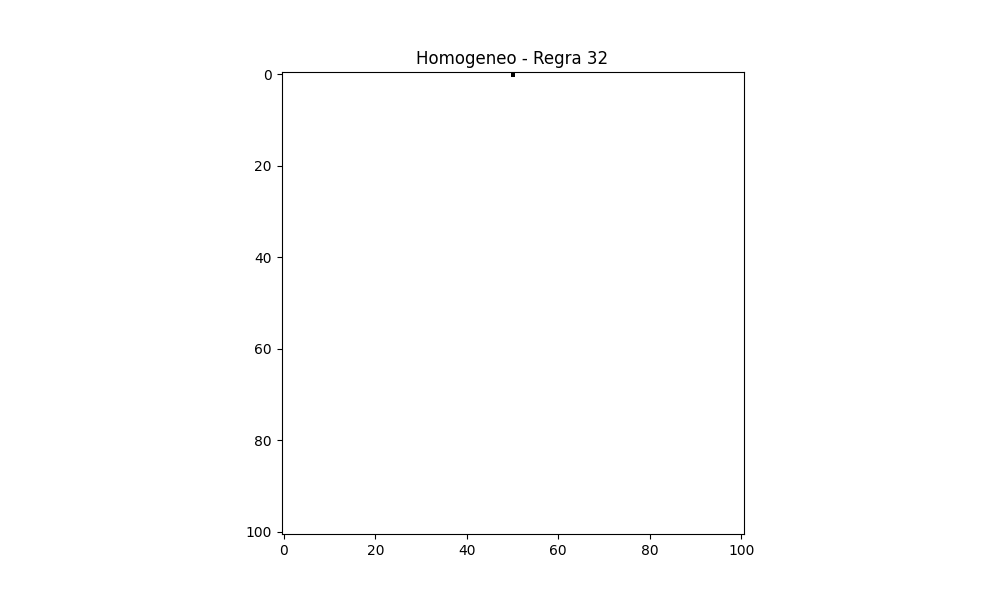
\includegraphics[width=0.75\textwidth]{figuras/graficos/Homogeneo_regra_32_tamanho_101_passos_100.png}
    \caption{Classe homogenea: Regra 32.}
    \label{fig:homogeneo-r32}
\end{figure}

\begin{figure}[H]
    \centering
    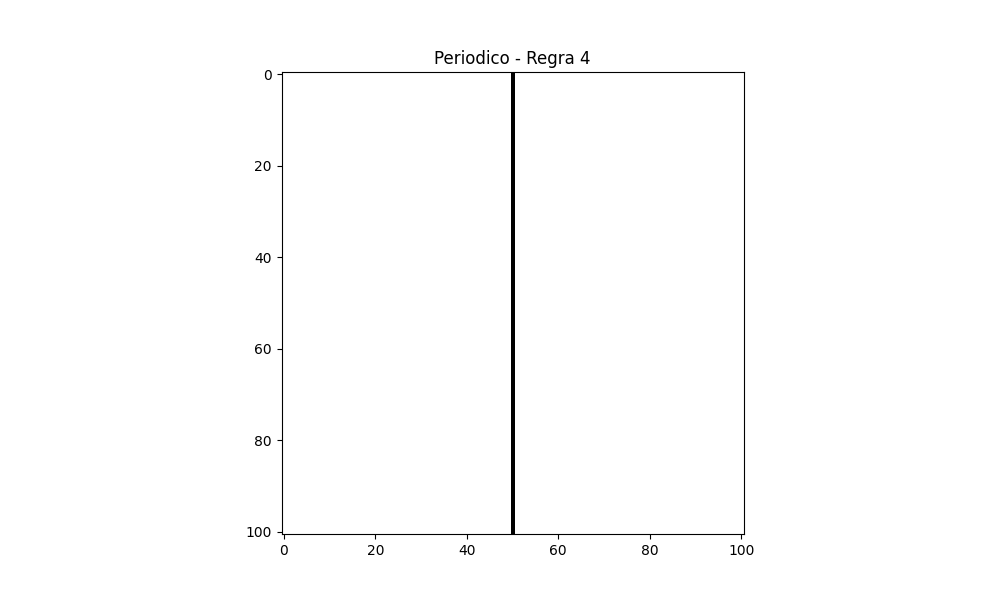
\includegraphics[width=0.75\textwidth]{figuras/graficos/Periodico_regra_4_tamanho_101_passos_100.png}
    \caption{Classe periodica: Regra 4.}
    \label{fig:periodico-r4}
\end{figure}

\begin{figure}[H]
    \centering
    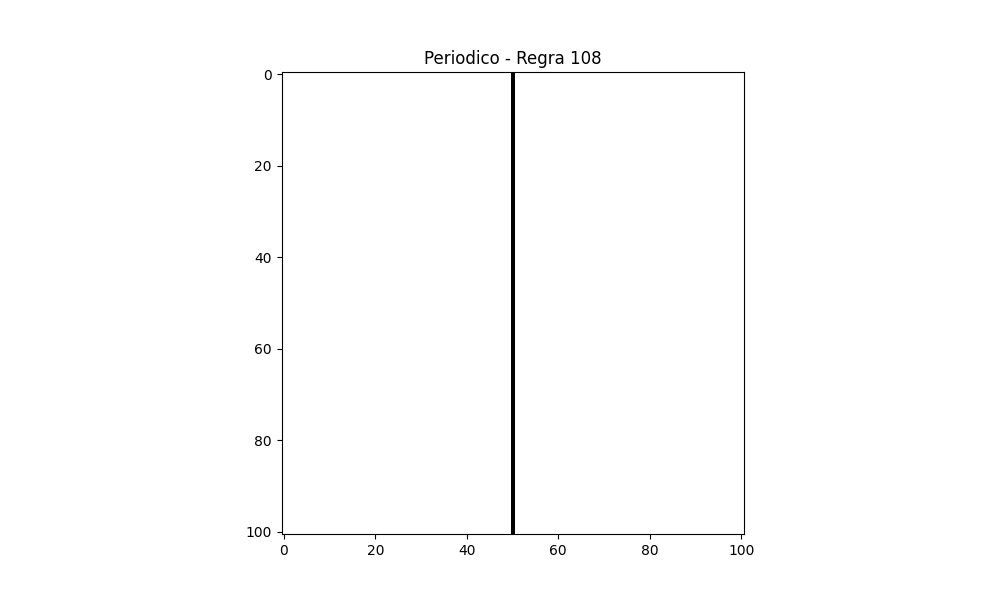
\includegraphics[width=0.75\textwidth]{figuras/graficos/Periodico_regra_108_tamanho_101_passos_100.png}
    \caption{Classe periodica: Regra 108.}
    \label{fig:periodico-r108}
\end{figure}

\begin{figure}[H]
    \centering
    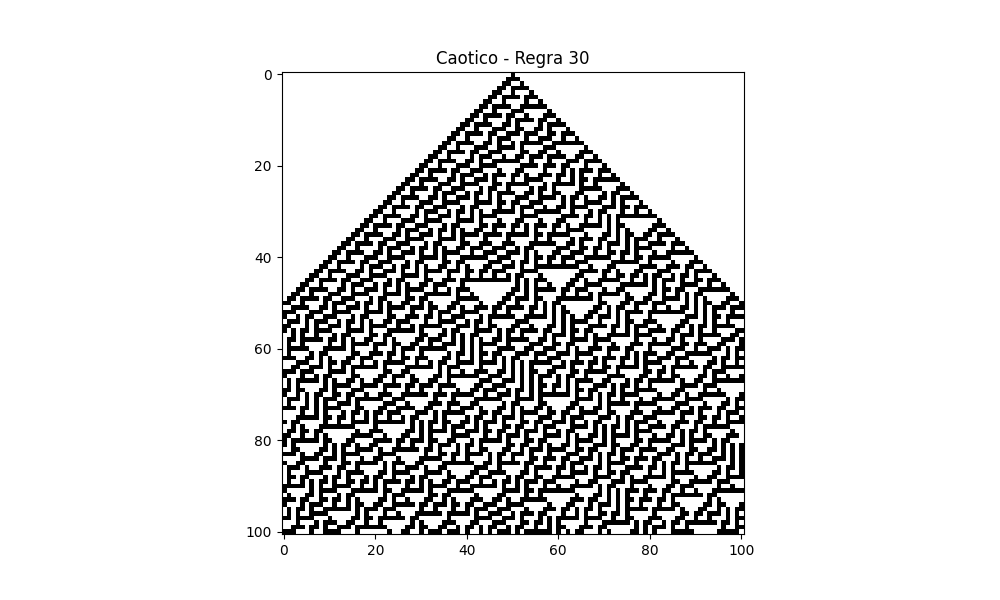
\includegraphics[width=0.75\textwidth]{figuras/graficos/Caotico_regra_30_tamanho_101_passos_100.png}
    \caption{Classe caotica: Regra 30.}
    \label{fig:caotico-r30}
\end{figure}

\begin{figure}[H]
    \centering
    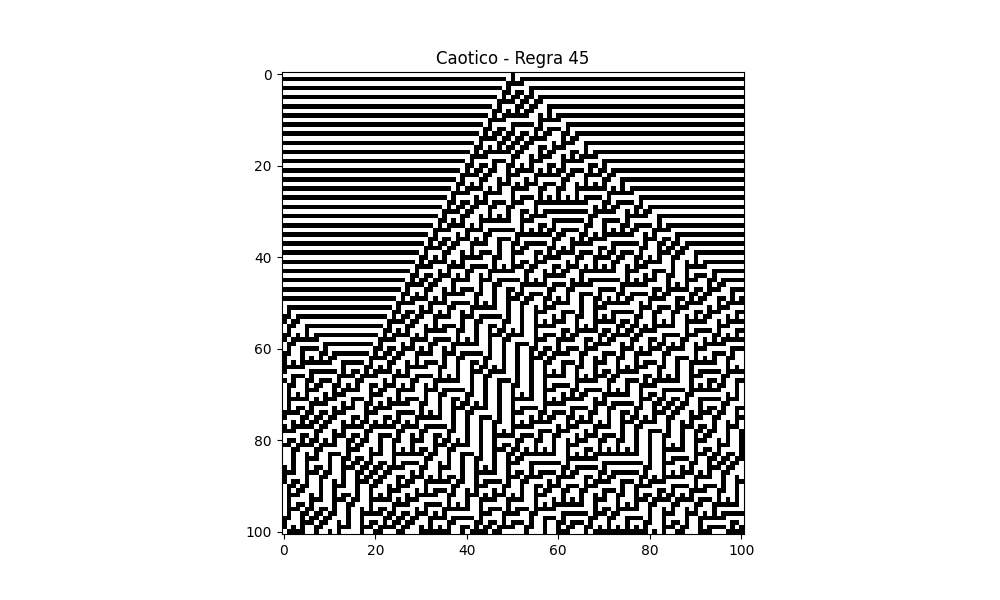
\includegraphics[width=0.75\textwidth]{figuras/graficos/Caotico_regra_45_tamanho_101_passos_100.png}
    \caption{Classe caotica: Regra 45.}
    \label{fig:caotico-r45}
\end{figure}

\begin{figure}[H]
    \centering
    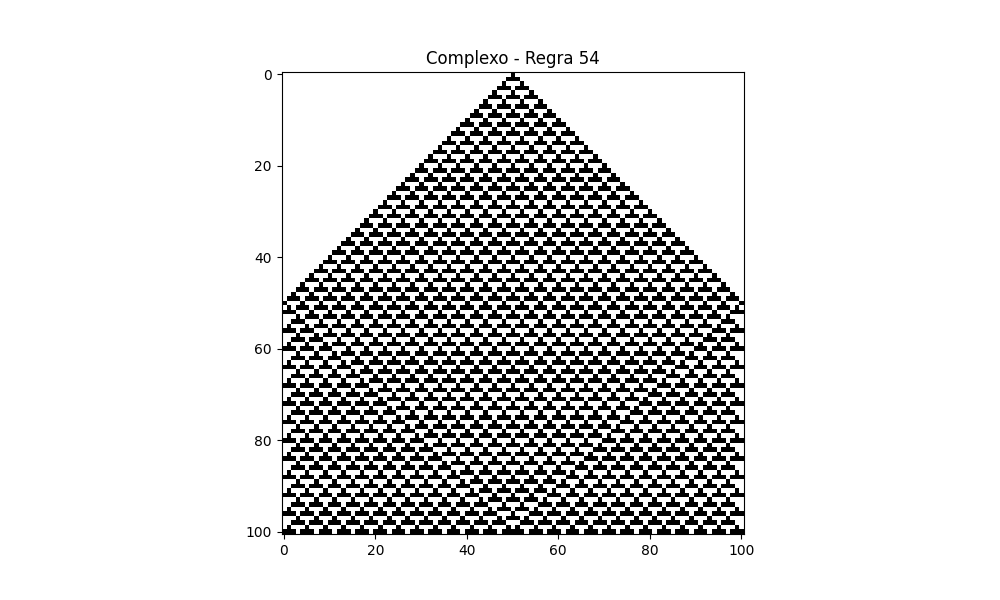
\includegraphics[width=0.75\textwidth]{figuras/graficos/Complexo_regra_54_tamanho_101_passos_100.png}
    \caption{Classe complexa: Regra 54.}
    \label{fig:complexo-r54}
\end{figure}

\begin{figure}[H]
    \centering
    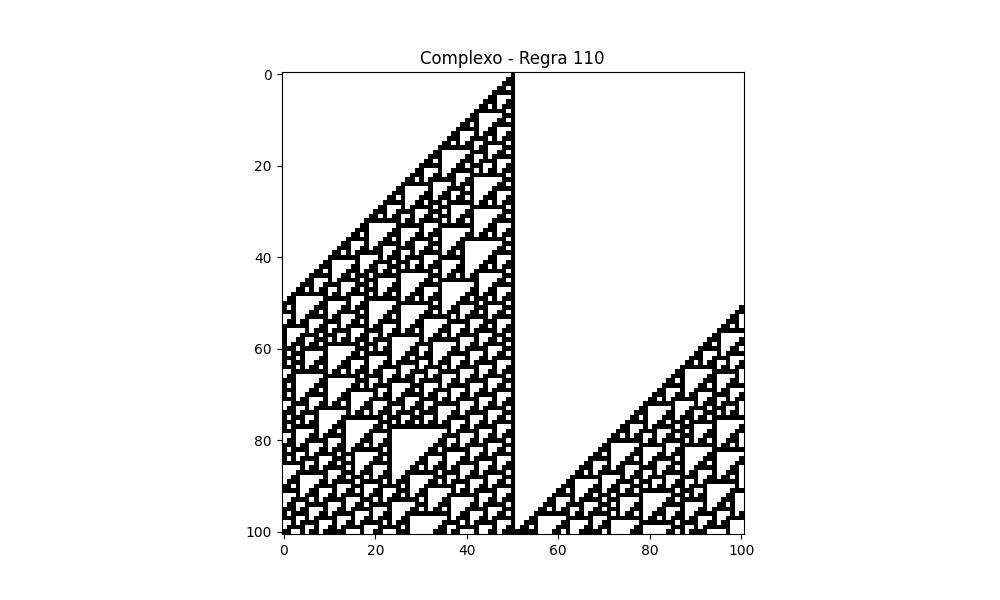
\includegraphics[width=0.75\textwidth]{figuras/graficos/Complexo_regra_110_tamanho_101_passos_100.png}
    \caption{Classe complexa: Regra 110.}
    \label{fig:complexo-r110}
\end{figure}

A classificacao visual e coerente com a literatura: as regras 0 e 32 convergem rapidamente para estados simples; 4 e 108 mantem padroes repetitivos; 30 e 45 exibem irregularidade espacial; e 54 e 110 apresentam estruturas localizadas e interacoes de maior complexidade.

\section{Metricas extraidas dos CSV}

A Tabela~\ref{tab:resumo-metricas-101-100} resume metricas para o conjunto \(tamanho=101\), \(passos=100\), calculadas diretamente dos dados de saida em CSV. Foram consideradas: densidade media de celulas ativas, densidade no ultimo passo e numero de ativos no ultimo passo.

\begin{table}[H]
\centering
\caption{Resumo quantitativo para \(tamanho=101\) e \(passos=100\).}
\label{tab:resumo-metricas-101-100}
\begin{tabular}{lccc}
\toprule
Regra & Densidade media & Densidade final & Ativos finais \\
\midrule
0   & 0.0001 & 0.0000 & 0  \\
32  & 0.0001 & 0.0000 & 0  \\
4   & 0.0099 & 0.0099 & 1  \\
108 & 0.0099 & 0.0099 & 1  \\
30  & 0.3862 & 0.5149 & 52 \\
45  & 0.4955 & 0.5446 & 55 \\
54  & 0.3777 & 0.7624 & 77 \\
110 & 0.2870 & 0.5149 & 52 \\
\bottomrule
\end{tabular}
\end{table}

Os resultados numericos reforcam a classificacao visual: regras homogeneas e periodicas apresentam baixissima atividade media, enquanto regras caoticas e complexas mantem atividade elevada ao longo da simulacao.

\section{Comparacao de tamanho de malha (passos=200)}

Para avaliar sensibilidade a escala, foram comparadas as regras 30, 45, 54 e 110 em dois tamanhos de malha (101 e 200), mantendo \(passos=200\).

\begin{table}[H]
\centering
\caption{Comparacao de densidade media para \(passos=200\).}
\label{tab:comparacao-tamanho-200}
\begin{tabular}{lcc}
\toprule
Regra & Densidade media (tam. 101) & Densidade media (tam. 200) \\
\midrule
30  & 0.4441 & 0.3799 \\
45  & 0.4953 & 0.4952 \\
54  & 0.4349 & 0.3769 \\
110 & 0.4273 & 0.2914 \\
\bottomrule
\end{tabular}
\end{table}

Observa-se que a Regra 45 permanece praticamente invariante em densidade media, enquanto as regras 30, 54 e 110 apresentam reducao de densidade media ao aumentar o tamanho da malha. Esse comportamento indica dependencia da dinamica global em relacao a escala espacial para algumas regras.

Como exemplo de configuracao de maior escala, a Figura~\ref{fig:escala-r110-200} apresenta a Regra 110 com \(tamanho=200\) e \(passos=200\).

\begin{figure}[H]
    \centering
    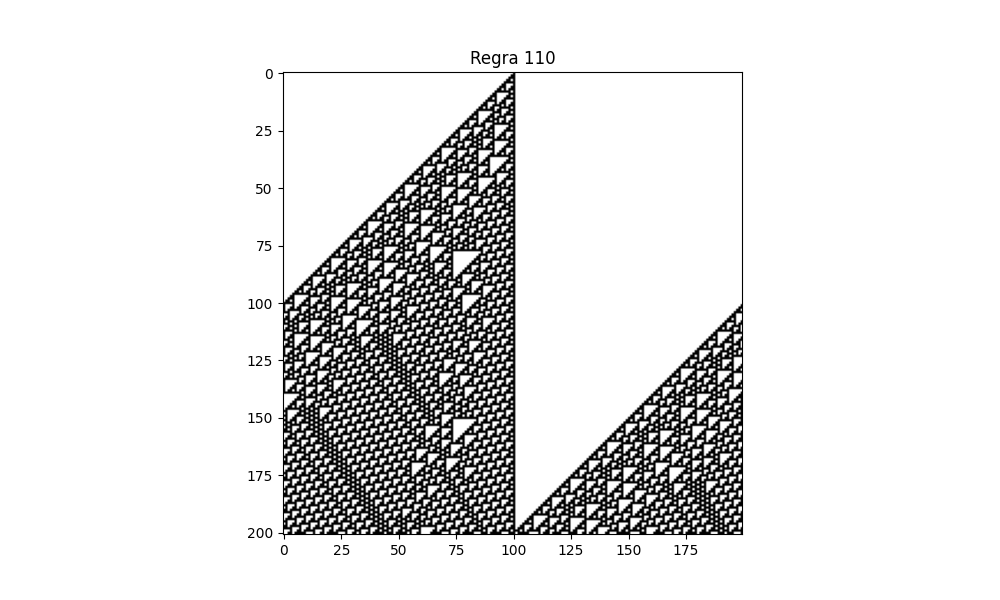
\includegraphics[width=0.85\textwidth]{figuras/graficos/regra_110_tamanho_200_passos_200.png}
    \caption{Regra 110 em maior escala (\(tamanho=200\), \(passos=200\)).}
    \label{fig:escala-r110-200}
\end{figure}

Para rastreabilidade dos parametros usados, exemplos de tabelas de entrada geradas automaticamente sao apresentados abaixo.

\begin{table}[H]
\centering
\caption{Tabela - Dados referentes a Homogeneo regra 0 tamanho 101 passos 100.}
\label{tab:Homogeneo_regra_0_tamanho_101_passos_100}
\begin{tabular}{ll}
\toprule
classe & Homogeneo \\
\midrule
regra & 0 \\
tamanho & 101 \\
passos & 100 \\
\bottomrule
\end{tabular}

\end{table}

\begin{table}[H]
\centering
\caption{Tabela - Dados referentes a Caotico regra 30 tamanho 101 passos 100.}
\label{tab:Caotico_regra_30_tamanho_101_passos_100}
\begin{tabular}{ll}
\toprule
classe & Caotico \\
\midrule
regra & 30 \\
tamanho & 101 \\
passos & 100 \\
\bottomrule
\end{tabular}

\end{table}

\begin{table}[H]
\centering
\caption{Tabela - Dados referentes a Complexo regra 110 tamanho 101 passos 100.}
\label{tab:Complexo_regra_110_tamanho_101_passos_100}
\begin{tabular}{ll}
\toprule
classe & Complexo \\
\midrule
regra & 110 \\
tamanho & 101 \\
passos & 100 \\
\bottomrule
\end{tabular}

\end{table}

